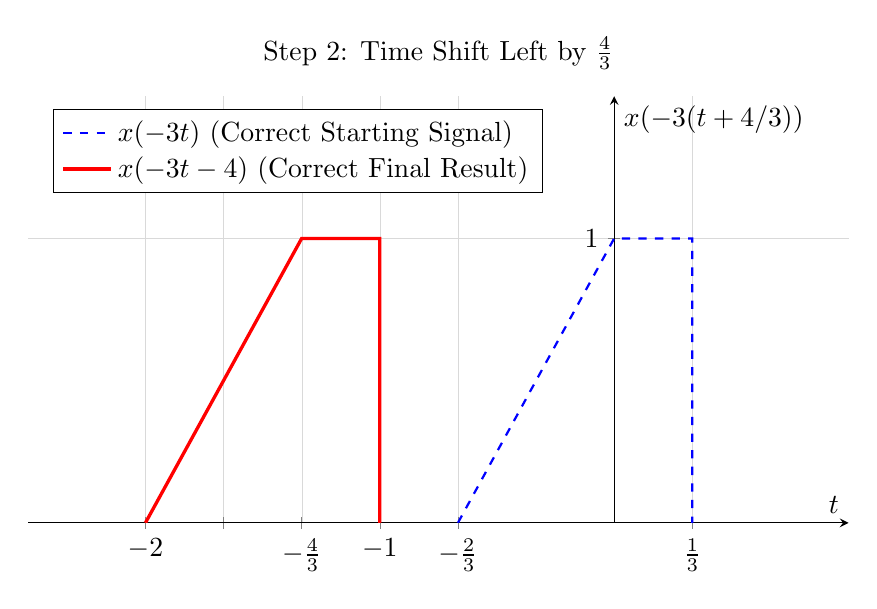
\begin{tikzpicture}
	\begin{axis}[
		% Set the overall style
		width=12cm,
		height=7cm,
		% Title and labels
		title={Step 2: Time Shift Left by $\frac{4}{3}$},
		xlabel={$t$},
		ylabel={$x(-3(t+4/3))$},
		% Position axes at the origin
		axis lines=middle,
		% Set axis limits for good spacing
		xmin=-2.5, xmax=1,
		ymin=0, ymax=1.5,
		% Set ticks at key fractional and integer points
		xtick={-2, -5/3, -4/3, -1, -2/3, 0, 1/3},
		xticklabels={$-2$,,$-\frac{4}{3}$,$-1$,$-\frac{2}{3}$,$0$,$\frac{1}{3}$},
		ytick={1},
		grid=major,
		grid style={line width=.1pt, draw=gray!30},
		legend pos=north west,
		legend cell align={left},
		]
		
		% Plot the CORRECT x(-3t) signal (dashed blue)
		\addplot[blue, dashed, thick] coordinates {
			(-2/3, 0) (0, 1) (1/3, 1) (1/3, 0)
		};
		\addlegendentry{$x(-3t)$ (Correct Starting Signal)};
		
		% Plot the CORRECT shifted signal (solid red)
		% This is x(-3t) shifted left by 4/3
		\addplot[red, very thick] coordinates {
			(-2, 0) (-4/3, 1) (-1, 1) (-1, 0)
		};
		\addlegendentry{$x(-3t - 4)$ (Correct Final Result)};
		
	\end{axis}
\end{tikzpicture}